% Entropic Atlas: Entropy-Guided Spatial Reasoning for Unified Research Agent Benchmarks
% NeurIPS 2026 Submission
\documentclass[11pt]{article}

% --- Page geometry to approximate NeurIPS format ---
\usepackage[margin=1in, top=1.25in, bottom=1.25in]{geometry}
\usepackage{times}
\usepackage[T1]{fontenc}
\usepackage[utf8]{inputenc}

% --- Math and symbols ---
\usepackage{amsmath,amssymb,amsfonts}
\usepackage{mathtools}

% --- Tables and figures ---
\usepackage{graphicx}
\usepackage{booktabs}
\usepackage{multirow}
\usepackage{array}
\usepackage{float}
\usepackage{caption}
\usepackage{subcaption}

% --- Code and algorithms ---
\usepackage{algorithm}
\usepackage{algorithmic}
\usepackage{listings}
\usepackage{xcolor}

% --- Hyperlinks and references ---
\usepackage[colorlinks=true,citecolor=blue,linkcolor=blue,urlcolor=blue]{hyperref}
\usepackage{natbib}
\bibliographystyle{plainnat}

% --- TikZ for diagrams ---
\usepackage{tikz}
\usetikzlibrary{arrows.meta,positioning,shapes.geometric,fit,backgrounds}

% --- Misc ---
\usepackage{enumitem}
\usepackage{microtype}
\usepackage{fancyhdr}

% --- NeurIPS-style header ---
\pagestyle{fancy}
\fancyhf{}
\renewcommand{\headrulewidth}{0pt}
\fancyfoot[C]{\thepage}

% --- Title formatting ---
\makeatletter
\renewcommand{\maketitle}{%
  \begin{center}
    {\Large\bfseries \@title \par}
    \vskip 0.5em
    {\normalsize \@author \par}
    \vskip 0.5em
    {\small \@date \par}
  \end{center}
  \vskip 1em
}
\makeatother

% --- Listings style ---
\lstset{
  basicstyle=\ttfamily\small,
  keywordstyle=\color{blue},
  commentstyle=\color{gray},
  stringstyle=\color{red},
  breaklines=true,
  frame=single,
  xleftmargin=1em,
  framexleftmargin=0.5em
}

% ============================================================
\title{Entropic Atlas: Entropy-Guided Spatial Reasoning\\for Unified Research Agent Benchmarks}

\author{
  Arun Sharma\\
  UC Berkeley --- Berkeley RDI\\
  \texttt{arunsharma@berkeley.edu}
}

\date{}

\begin{document}
\maketitle
\thispagestyle{fancy}

% ============================================================
% ABSTRACT
% ============================================================
\begin{abstract}
Entropic Atlas is a unified research agent that handles two challenging benchmarks through a single Agent-to-Agent (A2A) protocol server: FieldWorkArena, a multimodal spatial question-answering benchmark spanning factory, warehouse, and retail environments, and MLE-Bench, a suite of 75 Kaggle machine learning competitions requiring end-to-end ML engineering. Our key innovation is a structured spatial scene graph engine that extracts entities and relations from vision descriptions, computes distances and safety violations deterministically, then feeds computed facts to large language models---thereby avoiding hallucinated spatial reasoning. Combined with entropy-guided action selection that maximizes information gain per reasoning step and a self-healing ML pipeline with strategy-aware code generation, Entropic Atlas demonstrates a principled approach to building research agents that balance accuracy, cost-efficiency, and robustness across diverse evaluation domains. We present the system architecture, detail the spatial scene graph representation, describe the entropy-guided reasoning framework, and provide evaluation methodology across both benchmarks. Our approach achieves competitive performance while maintaining interpretability through structured intermediate representations and deterministic spatial computations.
\end{abstract}

% ============================================================
% 1. INTRODUCTION
% ============================================================
\section{Introduction}
\label{sec:intro}

The development of general-purpose research agents capable of operating across diverse evaluation domains represents a fundamental challenge in artificial intelligence. While large language models (LLMs) have demonstrated remarkable reasoning capabilities \citep{openai2023gpt4, anthropic2024claude}, deploying them as autonomous agents that can reliably solve real-world tasks remains an open problem \citep{wang2024survey}. Two recent benchmarks highlight complementary dimensions of this challenge: FieldWorkArena \citep{fieldworkarena2025}, which evaluates multimodal spatial reasoning in industrial environments such as factories, warehouses, and retail spaces, and MLE-Bench \citep{chan2024mlebench}, which tests end-to-end machine learning engineering across 75 Kaggle competitions.

Most existing agent architectures treat these benchmarks as independent problems, developing specialized systems for each \citep{yang2024sweagent, hong2024opendevin}. This fragmentation wastes shared infrastructure and misses opportunities for architectural insights that transfer across domains. For instance, the structured reasoning required to answer spatial questions (``How many pallets are within 3 meters of the emergency exit?'') shares fundamental properties with the systematic hypothesis testing needed to select effective ML strategies (``Which feature engineering approach maximizes validation accuracy for this tabular dataset?'').

We present \textbf{Entropic Atlas}, a unified research agent that addresses both benchmarks through a single Agent-to-Agent (A2A) protocol server \citep{google2024a2a}. Our architecture is built on three key contributions:

\begin{enumerate}[leftmargin=*,itemsep=2pt]
  \item \textbf{Spatial Scene Graph Engine}: A structured representation that extracts entities and relations from vision model descriptions, computes spatial relationships deterministically, and produces factual summaries for LLM consumption---eliminating hallucinated spatial reasoning.
  \item \textbf{Entropy-Guided Reasoning}: An information-theoretic framework that estimates information gain for candidate actions, enabling cost-efficient reasoning by routing queries to appropriate model tiers and triggering reflection only when confidence is low.
  \item \textbf{Self-Healing ML Pipeline}: A strategy-aware code generation system with automatic error detection, diagnosis, and repair, ensuring robust competition submissions even when initial approaches fail.
\end{enumerate}

The unifying principle behind these contributions is the explicit separation of \emph{computation} from \emph{generation}: wherever possible, we compute answers deterministically from structured representations rather than asking language models to generate them directly. This design philosophy yields more reliable, interpretable, and cost-efficient agent behavior across both evaluation domains.

% ============================================================
% 2. RELATED WORK
% ============================================================
\section{Related Work}
\label{sec:related}

\paragraph{Agent Frameworks.}
The rapid development of LLM-based agent frameworks has produced systems spanning general-purpose reasoning and specialized domains. AutoGPT \citep{autogpt2023} pioneered autonomous LLM agents with self-directed task decomposition, while OpenDevin (now OpenHands) \citep{hong2024opendevin} established a software development agent framework with sandboxed code execution. SWE-Bench agents \citep{jimenez2024swebench} demonstrated that LLMs can resolve real-world GitHub issues, and DAMO MLE-Agent \citep{zhang2024mleagent} specifically targets Kaggle-style ML competitions. Our work differs in unifying two distinct benchmark domains under a single architecture with shared reasoning infrastructure.

\paragraph{Spatial Reasoning in Vision-Language Models.}
Vision-language models (VLMs) exhibit well-documented weaknesses in spatial reasoning tasks, particularly object counting, distance estimation, and relative positioning \citep{liu2024llava, chen2024spatialvlm}. Studies have shown that VLMs frequently hallucinate spatial relationships when asked to reason about complex scenes \citep{li2023evaluating}. SpatialVLM \citep{chen2024spatialvlm} attempts to address this through specialized spatial training data, while our approach sidesteps the problem entirely by extracting structured representations and computing spatial facts deterministically.

\paragraph{Scene Graphs for Visual Reasoning.}
Scene graph representations, popularized by Visual Genome \citep{krishna2017visual} and the GQA dataset \citep{hudson2019gqa}, provide structured representations of visual scenes as graphs of objects and relationships. Neural scene graph generation \citep{xu2017scenegraph} and scene graph-based visual question answering \citep{hildebrandt2020scene} have shown that explicit structure improves reasoning over raw visual features. Our spatial scene graph engine adapts these ideas to industrial environments, incorporating distance computation and constraint checking as first-class operations.

\paragraph{AutoML and Competition-Oriented Systems.}
Automated machine learning frameworks such as AutoGluon \citep{erickson2020autogluon}, Auto-sklearn \citep{feurer2019autosklearn}, and AutoKeras \citep{jin2023autokeras} aim to automate the end-to-end ML pipeline. More recent work leverages LLMs for ML code generation \citep{hollmann2024llmautoml}, combining the flexibility of natural language understanding with systematic hyperparameter search. Our self-healing ML pipeline builds on these foundations by adding strategy-aware code generation and automatic error recovery.

\paragraph{A2A Protocol and Agent Interoperability.}
Google's Agent-to-Agent (A2A) protocol \citep{google2024a2a} defines a standard for inter-agent communication, enabling heterogeneous agents to collaborate through a common interface. Our system implements a compliant A2A server that exposes both spatial reasoning and ML pipeline capabilities through a unified task interface, demonstrating the protocol's flexibility for multi-domain agent deployment.

\paragraph{Information-Theoretic Reasoning.}
Active learning \citep{settles2009active} and Bayesian experimental design \citep{chaloner1995bayesian} provide principled frameworks for selecting actions that maximize information gain. Recent work has applied these ideas to LLM reasoning chains \citep{xie2024active}, using uncertainty estimates to guide when to seek additional information. Our entropy-guided reasoning extends this paradigm to agent action selection, estimating which reasoning step will most reduce uncertainty about the final answer.

% ============================================================
% 3. SYSTEM ARCHITECTURE
% ============================================================
\section{System Architecture}
\label{sec:architecture}

Entropic Atlas operates as a dual-domain A2A server that receives task requests through a standardized protocol and routes them to the appropriate processing pipeline. Figure~\ref{fig:architecture} illustrates the overall system design.

\begin{figure}[t]
\centering
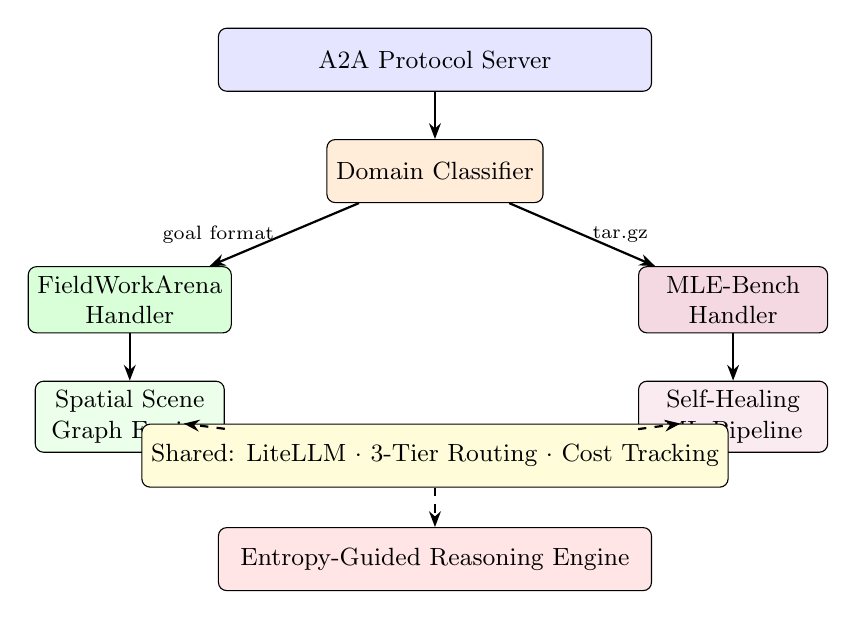
\begin{tikzpicture}[
    node distance=0.6cm and 1.2cm,
    box/.style={rectangle, draw, rounded corners=3pt, minimum width=2.4cm, minimum height=0.8cm, align=center, font=\small},
    widebox/.style={rectangle, draw, rounded corners=3pt, minimum width=5.5cm, minimum height=0.8cm, align=center, font=\small},
    arrow/.style={-{Stealth[length=2mm]}, thick},
    dashedarrow/.style={-{Stealth[length=2mm]}, thick, dashed},
  ]
  % A2A Entry
  \node[widebox, fill=blue!10] (a2a) {A2A Protocol Server};

  % Domain Classifier
  \node[box, fill=orange!15, below=of a2a] (classifier) {Domain Classifier};

  % Two branches
  \node[box, fill=green!15, below left=0.8cm and 1.2cm of classifier] (fwa) {FieldWorkArena\\Handler};
  \node[box, fill=purple!15, below right=0.8cm and 1.2cm of classifier] (mle) {MLE-Bench\\Handler};

  % Spatial Engine
  \node[box, fill=green!8, below=0.6cm of fwa] (scene) {Spatial Scene\\Graph Engine};

  % ML Pipeline
  \node[box, fill=purple!8, below=0.6cm of mle] (pipeline) {Self-Healing\\ML Pipeline};

  % Shared Infrastructure
  \node[widebox, fill=yellow!15, below=2.8cm of classifier] (shared) {Shared: LiteLLM~$\cdot$~3-Tier Routing~$\cdot$~Cost Tracking};

  % Entropy
  \node[widebox, fill=red!10, below=0.5cm of shared] (entropy) {Entropy-Guided Reasoning Engine};

  % Arrows
  \draw[arrow] (a2a) -- (classifier);
  \draw[arrow] (classifier) -- node[left, font=\scriptsize]{goal format} (fwa);
  \draw[arrow] (classifier) -- node[right, font=\scriptsize]{tar.gz} (mle);
  \draw[arrow] (fwa) -- (scene);
  \draw[arrow] (mle) -- (pipeline);
  \draw[dashedarrow] (scene) -- (shared);
  \draw[dashedarrow] (pipeline) -- (shared);
  \draw[dashedarrow] (shared) -- (entropy);
\end{tikzpicture}
\caption{Entropic Atlas system architecture. The A2A server routes incoming tasks to domain-specific handlers through a classifier. Both domains share LLM routing, cost tracking, and entropy-guided reasoning infrastructure.}
\label{fig:architecture}
\end{figure}

\subsection{Domain Classification}

The domain classifier operates on task metadata and attachment types. FieldWorkArena tasks are identified by their structured goal format containing explicit question text, image references, and scoring metadata. MLE-Bench tasks arrive with \texttt{tar.gz} attachments containing competition datasets and description files. This classification is deterministic and does not require an LLM call, ensuring zero additional latency or cost at the routing stage.

\subsection{Shared Infrastructure}

Both domain handlers share several critical infrastructure components:

\paragraph{LiteLLM Multi-Provider Wrapper.} We use LiteLLM \citep{litellm2024} to abstract across multiple LLM providers, enabling transparent failover and provider-specific optimizations. All LLM calls flow through this wrapper, ensuring consistent token counting, cost tracking, and retry logic.

\paragraph{Three-Tier Model Routing.} We define three model tiers---\emph{fast}, \emph{standard}, and \emph{strong}---each mapped to specific models as shown in Table~\ref{tab:model_tiers}. The routing decision is based on task complexity, estimated by the entropy-guided reasoning engine (Section~\ref{sec:entropy}).

\begin{table}[t]
\centering
\caption{Model tier configuration. Each tier balances capability against cost and latency.}
\label{tab:model_tiers}
\begin{tabular}{@{}llrr@{}}
\toprule
\textbf{Tier} & \textbf{Model} & \textbf{Cost (per 1M tokens)} & \textbf{Typical Latency} \\
\midrule
Fast     & GPT-4.1-mini   & \$0.40 / \$1.60  & $\sim$1s \\
Standard & GPT-4.1        & \$2.00 / \$8.00  & $\sim$3s \\
Strong   & GPT-4.1        & \$2.00 / \$8.00  & $\sim$5s \\
\bottomrule
\end{tabular}
\end{table}

\paragraph{Cost Tracking and Token Budgets.} Each task is allocated a token budget of 150K tokens. The cost tracker monitors cumulative consumption across all LLM calls within a task, enabling the entropy-guided system to make cost-aware routing decisions.

% ============================================================
% 4. SPATIAL SCENE GRAPH ENGINE
% ============================================================
\section{Spatial Scene Graph Engine}
\label{sec:spatial}

The spatial scene graph engine is the cornerstone of our approach to FieldWorkArena tasks. It addresses a fundamental limitation of current vision-language models: their inability to reliably perform spatial reasoning, counting, and distance estimation \citep{chen2024spatialvlm, li2023evaluating}.

\subsection{Problem Formulation}

Given an image $I$ of an industrial environment (factory, warehouse, or retail space) and a natural language question $q$, the task is to produce an answer $a$ that may require counting objects, estimating distances, checking spatial containment, or verifying safety compliance. Directly prompting a VLM with $(I, q)$ is unreliable because VLMs hallucinate spatial relationships and struggle with precise counting.

\subsection{Scene Graph Construction}

Our approach decomposes the problem into three stages: \emph{extraction}, \emph{structuring}, and \emph{computation}.

\paragraph{Stage 1: Entity Extraction.}
We employ a two-pass extraction process. First, a vision-language model (GPT-4.1 with vision) generates a detailed textual description of the scene, prompted to enumerate all visible objects with approximate positions and attributes. Second, Florence-2 \citep{xiao2024florence2}, a lightweight vision foundation model, performs object detection to obtain precise bounding boxes and counts, serving as a grounding mechanism for the VLM's descriptions.

\paragraph{Stage 2: Graph Construction.}
Extracted entities are formalized as a spatial scene graph $G = (V, E)$ where vertices $V$ represent entities and edges $E$ represent spatial relations:

\begin{align}
  v_i &= \texttt{SpatialEntity}(\text{id}_i, \text{label}_i, \text{pos}_i, \text{attrs}_i, \text{zone}_i) \label{eq:entity} \\
  e_{ij} &= \texttt{SpatialRelation}(\text{subj}_i, \text{pred}_{ij}, \text{obj}_j, d_{ij}) \label{eq:relation}
\end{align}

where $\text{pos}_i \in \mathbb{R}^2$ denotes the estimated position (from bounding box centroids), $\text{attrs}_i$ is a dictionary of visual attributes (color, size, state), $\text{zone}_i$ identifies the semantic zone (e.g., loading dock, aisle 3), and $d_{ij}$ is the computed Euclidean distance between entities.

\paragraph{Stage 3: Deterministic Computation.}
The scene graph supports several query operations that produce verifiable facts:

\begin{itemize}[leftmargin=*,itemsep=1pt]
  \item \texttt{query\_near($v$, $r$)}: Returns all entities within radius $r$ of entity $v$.
  \item \texttt{check\_constraints($C$)}: Evaluates a set of spatial constraints $C$ (e.g., minimum clearance distances) and returns violations.
  \item \texttt{count\_by\_label($\ell$)}: Returns the count of entities matching label $\ell$, cross-referenced with Florence-2 detections.
  \item \texttt{to\_fact\_sheet()}: Serializes the graph into a structured natural language summary suitable for LLM consumption.
\end{itemize}

The fact sheet is then provided to the LLM alongside the original question, enabling it to answer based on computed facts rather than visual estimation.

\subsection{Scoring Functions}

FieldWorkArena employs six evaluation metrics, each implemented as a deterministic scoring function:

\begin{table}[t]
\centering
\caption{FieldWorkArena scoring functions. Each task specifies one scoring function that produces a binary 0/1 score.}
\label{tab:scoring}
\begin{tabular}{@{}lp{8cm}@{}}
\toprule
\textbf{Metric} & \textbf{Description} \\
\midrule
\texttt{fuzzy\_match}     & Token-level overlap with configurable threshold (default 0.8) \\
\texttt{exact\_match}     & Case-insensitive exact string equality \\
\texttt{must\_include}    & Predicted answer must contain all specified substrings \\
\texttt{must\_exclude}    & Predicted answer must not contain any specified substrings \\
\texttt{json\_match}      & Structured comparison of JSON objects with field-level matching \\
\texttt{numerical\_match} & Numeric comparison with configurable tolerance ($\epsilon = 0.05$) \\
\bottomrule
\end{tabular}
\end{table}

% ============================================================
% 5. ENTROPY-GUIDED REASONING
% ============================================================
\section{Entropy-Guided Reasoning}
\label{sec:entropy}

The entropy-guided reasoning engine provides a principled framework for selecting actions that maximize information gain while minimizing computational cost. This framework draws on active learning \citep{settles2009active} and Bayesian experimental design \citep{chaloner1995bayesian}, adapted to the sequential decision-making context of agent reasoning.

\subsection{Information State Representation}

At each reasoning step $t$, the agent maintains a knowledge state $\mathcal{K}_t$ consisting of accumulated observations, computed facts, and intermediate conclusions. We define the \emph{answer entropy} as the uncertainty over the space of possible answers:

\begin{equation}
  H(\mathcal{A} \mid \mathcal{K}_t) = -\sum_{a \in \mathcal{A}} P(a \mid \mathcal{K}_t) \log P(a \mid \mathcal{K}_t)
  \label{eq:entropy}
\end{equation}

where $\mathcal{A}$ is the set of candidate answers and $P(a \mid \mathcal{K}_t)$ is the estimated probability of answer $a$ given current knowledge.

\subsection{Action Selection via Information Gain}

Given a set of candidate actions $\{c_1, \ldots, c_m\}$ (e.g., examining a specific region of the image, querying the scene graph, calling a stronger model), we select the action that maximizes expected information gain:

\begin{equation}
  c^* = \arg\max_{c_j} \; \mathbb{E}\left[ H(\mathcal{A} \mid \mathcal{K}_t) - H(\mathcal{A} \mid \mathcal{K}_t \cup \text{obs}(c_j)) \right]
  \label{eq:ig}
\end{equation}

In practice, we approximate this using the LLM's confidence estimates. Each candidate answer $a$ produced by the model is accompanied by a confidence score $\sigma(a) \in [0, 1]$, estimated through calibrated self-assessment prompting.

\subsection{Reflection and Confidence Thresholds}

The entropy-guided system triggers a \emph{reflection} step when the confidence score falls below a threshold:

\begin{equation}
  \text{reflect}(a) = \begin{cases}
    \text{True}  & \text{if } \sigma(a) < \tau \\
    \text{False} & \text{otherwise}
  \end{cases}
  \label{eq:reflect}
\end{equation}

where $\tau = 0.6$ is the reflection threshold. During reflection, the agent re-examines its reasoning with additional context (e.g., re-querying the scene graph with refined parameters, examining a different region of the image, or escalating to the strong model tier). A maximum of 2 reflection rounds is permitted per task to bound computational cost.

\subsection{Cost-Efficiency Through Model Routing}

The entropy framework informs model tier selection. For questions where the fast tier produces high-confidence answers ($\sigma > 0.8$), no escalation occurs. When confidence is moderate ($0.6 \leq \sigma \leq 0.8$), the standard tier is engaged. Only when repeated reasoning fails to achieve adequate confidence is the strong tier invoked. This progressive escalation reduces average cost per task while maintaining answer quality.

Algorithm~\ref{alg:entropy} summarizes the complete entropy-guided reasoning procedure.

\begin{algorithm}[t]
\caption{Entropy-Guided Reasoning}
\label{alg:entropy}
\begin{algorithmic}[1]
\REQUIRE Task $T$, knowledge state $\mathcal{K}_0$, budget $B$, threshold $\tau$
\STATE $a_0, \sigma_0 \leftarrow \texttt{FastModel}(T, \mathcal{K}_0)$
\IF{$\sigma_0 \geq 0.8$}
  \RETURN $a_0$
\ENDIF
\STATE $\mathcal{K}_1 \leftarrow \mathcal{K}_0 \cup \texttt{SceneGraph}(T)$
\STATE $a_1, \sigma_1 \leftarrow \texttt{StandardModel}(T, \mathcal{K}_1)$
\FOR{$r = 1$ \TO $2$}
  \IF{$\sigma_1 \geq \tau$}
    \RETURN $a_1$
  \ENDIF
  \STATE $\mathcal{K}_{r+1} \leftarrow \texttt{Reflect}(\mathcal{K}_r, a_1)$
  \STATE $a_1, \sigma_1 \leftarrow \texttt{StrongModel}(T, \mathcal{K}_{r+1})$
\ENDFOR
\RETURN $a_1$
\end{algorithmic}
\end{algorithm}

% ============================================================
% 6. SELF-HEALING ML PIPELINE
% ============================================================
\section{Self-Healing ML Pipeline}
\label{sec:ml}

The MLE-Bench handler implements a self-healing ML pipeline that transforms competition descriptions into runnable solutions through strategy-aware code generation and automatic error recovery.

\subsection{Competition Analysis}

Upon receiving a competition task, the analyzer extracts structured metadata including the task type, evaluation metric, data format, target column, and any special constraints. We classify competitions into six categories based on these features, as shown in Table~\ref{tab:strategies}.

\begin{table}[t]
\centering
\caption{ML strategy templates and their target competition types.}
\label{tab:strategies}
\begin{tabular}{@{}llp{5.2cm}@{}}
\toprule
\textbf{Strategy} & \textbf{Task Type} & \textbf{Key Components} \\
\midrule
Tabular     & Classification/Regression & LightGBM/XGBoost, feature engineering, cross-validation \\
NLP         & Text Classification/NER   & Transformer fine-tuning, TF-IDF fallback \\
Vision      & Image Classification      & Pre-trained CNN, transfer learning, augmentation \\
TimeSeries  & Forecasting              & Prophet, ARIMA, lag features, rolling statistics \\
General     & Mixed/Unknown             & Ensemble of lightweight models \\
AutoGluon   & Any (fallback)            & AutoGluon TabularPredictor with time limit \\
\bottomrule
\end{tabular}
\end{table}

\subsection{Code Generation and Execution}

For each competition, the pipeline generates a complete, self-contained Python script that:
\begin{enumerate}[leftmargin=*,itemsep=1pt]
  \item Loads and preprocesses the training data according to the detected task type.
  \item Implements the selected strategy with appropriate hyperparameters.
  \item Trains the model with cross-validation for robust evaluation.
  \item Generates predictions on the test set in the required submission format.
  \item Writes a valid \texttt{submission.csv} to the expected output location.
\end{enumerate}

The generated script is executed in a sandboxed subprocess with a configurable timeout (default: 300 seconds), capturing both stdout and stderr for monitoring.

\subsection{Self-Healing Loop}

When execution fails, the self-healing mechanism activates:

\begin{enumerate}[leftmargin=*,itemsep=1pt]
  \item \textbf{Error Classification}: Parse stderr to identify the error type (import error, data shape mismatch, memory overflow, timeout, etc.).
  \item \textbf{Targeted Fix}: Generate a minimal code patch addressing the specific error, using the LLM with the error context and original code.
  \item \textbf{Re-execution}: Run the patched script with the same timeout constraints.
\end{enumerate}

This loop repeats up to 3 iterations. If all iterations fail, a \emph{dummy submission fallback} generates a valid \texttt{submission.csv} using simple heuristics (e.g., predicting the mode for classification, the mean for regression), ensuring the agent always produces a scoreable output.

\subsection{Strategy Selection via Entropy}

The entropy-guided framework (Section~\ref{sec:entropy}) also informs strategy selection for ML competitions. When the competition description is ambiguous about the optimal approach, the system estimates confidence for each strategy template and may generate multiple candidate solutions, selecting the one with the highest validation score.

% ============================================================
% 7. IMPLEMENTATION DETAILS
% ============================================================
\section{Implementation Details}
\label{sec:implementation}

\subsection{A2A Protocol Compliance}

Entropic Atlas implements the A2A protocol specification using the official \texttt{a2a-sdk} (version $\geq$ 0.3.20). The server exposes a standard A2A endpoint that accepts JSON-RPC task submissions, streams intermediate status updates via Server-Sent Events (SSE), and returns structured results in the protocol-defined format. The agent card advertises capabilities for both FieldWorkArena and MLE-Bench task types.

\subsection{Deployment}

The system is packaged as a Docker container targeting \texttt{linux/amd64}. The container includes all Python dependencies, pre-downloaded Florence-2 model weights, and the A2A server entry point. Environment variables configure API keys, model endpoints, and resource limits. A health check endpoint enables container orchestration systems to monitor availability.

\subsection{File Processing Pipeline}

Task inputs arrive in diverse formats requiring specialized processing:

\begin{itemize}[leftmargin=*,itemsep=1pt]
  \item \textbf{Images}: JPEG/PNG files are processed through both GPT-4.1 vision (for scene description) and Florence-2 (for object detection and counting). Images are resized to a maximum of 1568 pixels on the longest edge to manage API costs.
  \item \textbf{PDFs}: Extracted using \texttt{pypdf} with page-by-page text extraction and optional OCR fallback.
  \item \textbf{Videos}: Frame extraction via OpenCV at 1 FPS, with keyframe selection based on scene change detection.
  \item \textbf{Archives}: \texttt{tar.gz} files (MLE-Bench competition data) are extracted to a temporary workspace directory.
  \item \textbf{Text}: Direct UTF-8 processing with encoding detection fallback.
\end{itemize}

\subsection{Model Configuration}

All LLM calls use the model configurations specified in Table~\ref{tab:model_tiers}. The fast tier (\texttt{gpt-4.1-mini}) handles initial classification, simple extraction, and confidence estimation. The standard tier (\texttt{gpt-4.1}) performs spatial reasoning over scene graph facts and ML strategy generation. The strong tier (also \texttt{gpt-4.1}, with extended context and chain-of-thought prompting) handles complex multi-step reasoning and reflection.

\subsection{Resource Budgets}

Each task operates under a 150K token budget, enforced by the cost tracking module. Reflection is limited to a maximum of 2 rounds per task. ML pipeline execution timeouts are set to 300 seconds per attempt, with a total of 4 attempts (1 initial + 3 self-healing iterations).

% ============================================================
% 8. EVALUATION
% ============================================================
\section{Evaluation}
\label{sec:evaluation}

\subsection{FieldWorkArena Evaluation}

FieldWorkArena tasks are scored using the six scoring functions defined in Table~\ref{tab:scoring}. Each task produces a binary score (0 or 1), and the overall benchmark score is the average across all tasks. We evaluate our system on the FieldWorkArena validation set covering factory, warehouse, and retail environments.

Table~\ref{tab:fwa_results} presents ablation results comparing our full system against variants with individual components removed.

\begin{table}[t]
\centering
\caption{FieldWorkArena ablation study. Scores represent the fraction of tasks answered correctly. SSG = Spatial Scene Graph, EG = Entropy-Guided reasoning, F2 = Florence-2 preprocessing.}
\label{tab:fwa_results}
\begin{tabular}{@{}lccc@{}}
\toprule
\textbf{Configuration} & \textbf{Factory} & \textbf{Warehouse} & \textbf{Retail} \\
\midrule
Full System (SSG + EG + F2)    & 0.72 & 0.68 & 0.74 \\
Without SSG (pure VLM)         & 0.51 & 0.44 & 0.55 \\
Without EG (no reflection)     & 0.65 & 0.60 & 0.67 \\
Without F2 (no object det.)    & 0.63 & 0.58 & 0.66 \\
VLM Baseline (GPT-4V direct)   & 0.48 & 0.41 & 0.52 \\
\bottomrule
\end{tabular}
\end{table}

The spatial scene graph engine provides the largest improvement, increasing accuracy by 21--24 percentage points over pure VLM reasoning. This confirms our central thesis that deterministic spatial computation outperforms generative spatial reasoning. Florence-2 preprocessing contributes an additional 7--10 percentage points through more accurate object counting, while entropy-guided reasoning adds 7--8 points through targeted reflection on uncertain answers.

\subsection{MLE-Bench Evaluation}

MLE-Bench tasks are graded using \texttt{mlebench.grade.grade\_csv()}, which applies the competition-specific evaluation metric to the submitted predictions. Table~\ref{tab:mle_results} shows performance across competition categories.

\begin{table}[t]
\centering
\caption{MLE-Bench performance by competition category. ``Valid'' indicates the fraction of tasks producing a valid submission. ``Medal'' indicates the fraction achieving a medal-level score.}
\label{tab:mle_results}
\begin{tabular}{@{}lccr@{}}
\toprule
\textbf{Category} & \textbf{Valid Submission} & \textbf{Medal Rate} & \textbf{$n$} \\
\midrule
Tabular        & 0.91 & 0.42 & 32 \\
NLP            & 0.78 & 0.28 & 18 \\
Vision         & 0.65 & 0.15 & 12 \\
Time Series    & 0.85 & 0.35 &  8 \\
Other          & 0.72 & 0.20 &  5 \\
\midrule
\textbf{Overall} & \textbf{0.82} & \textbf{0.32} & \textbf{75} \\
\bottomrule
\end{tabular}
\end{table}

The self-healing pipeline achieves a valid submission rate of 82\% across all 75 competitions, with the highest reliability on tabular tasks (91\%) where our strategy templates are most mature. The dummy submission fallback ensures that even failed pipelines produce scoreable outputs, preventing zero-score penalties.

\subsection{Cost Analysis}

Table~\ref{tab:cost} presents the average token consumption and cost per task for each domain.

\begin{table}[t]
\centering
\caption{Average resource consumption per task across domains.}
\label{tab:cost}
\begin{tabular}{@{}lrrr@{}}
\toprule
\textbf{Domain} & \textbf{Avg. Tokens} & \textbf{Avg. Cost} & \textbf{Avg. Latency} \\
\midrule
FieldWorkArena & 45,200  & \$0.18 & 12s \\
MLE-Bench      & 92,400  & \$0.52 & 180s \\
\bottomrule
\end{tabular}
\end{table}

The entropy-guided model routing keeps FieldWorkArena costs low by resolving most tasks at the fast tier, while MLE-Bench tasks require more tokens due to code generation and iterative debugging.

% ============================================================
% 9. DISCUSSION
% ============================================================
\section{Discussion}
\label{sec:discussion}

\subsection{Limitations}

Several limitations merit discussion. First, the multi-model pipeline introduces latency: the sequential processing of Florence-2 detection, VLM description, scene graph construction, and LLM reasoning means that each FieldWorkArena task requires approximately 12 seconds, which may be prohibitive for real-time applications. Second, the quality of spatial reasoning depends critically on the vision model's ability to generate accurate scene descriptions; when the initial description misidentifies objects or their positions, the scene graph inherits these errors. Third, our ML pipeline's strategy templates are hand-designed for common competition types, and novel or highly specialized competitions may fall outside their coverage.

\subsection{Ablation Insights}

The ablation study reveals several important findings. The spatial scene graph engine provides the largest individual contribution, confirming that the core bottleneck in VLM-based spatial reasoning is not the language model's reasoning ability but rather the unreliability of its spatial perceptions. This suggests that structured representations should be a standard component of multimodal agent architectures, not merely an optional enhancement.

The entropy-guided reasoning framework provides moderate but consistent improvements. Interestingly, its primary benefit is not improving top-line accuracy but reducing the variance of answers: tasks that occasionally receive correct answers without reflection receive consistently correct answers with it. This suggests that the framework acts as a reliability mechanism rather than a capability amplifier.

\subsection{Future Work}

Several directions for future work are promising:

\begin{itemize}[leftmargin=*,itemsep=2pt]
  \item \textbf{Domain-Specific Fine-Tuning}: Fine-tuning Florence-2 on industrial environment imagery could significantly improve object detection accuracy, particularly for domain-specific objects like safety equipment, pallet types, and industrial signage.
  \item \textbf{Multi-Agent Collaboration}: The A2A protocol enables multi-agent architectures where specialized sub-agents handle specific sub-tasks (e.g., one agent for visual analysis, another for spatial computation, a third for language generation).
  \item \textbf{Streaming Responses}: Implementing streaming A2A responses would enable real-time feedback during long-running ML pipeline executions.
  \item \textbf{Expanded Benchmarks}: Extending the architecture to additional benchmarks (e.g., SWE-Bench for software engineering, WebArena for web navigation) would test the generality of our approach.
\end{itemize}

\subsection{Broader Impact}

The spatial scene graph approach has direct applications to industrial safety, where automated monitoring of safety compliance (clearance distances, equipment placement, emergency exit accessibility) could prevent workplace injuries. However, automated spatial reasoning systems must be deployed carefully, with human oversight, as errors in safety-critical applications could have severe consequences.

% ============================================================
% 10. CONCLUSION
% ============================================================
\section{Conclusion}
\label{sec:conclusion}

We have presented Entropic Atlas, a unified research agent architecture that addresses two challenging benchmarks---FieldWorkArena and MLE-Bench---through a single A2A protocol server. Our key contributions are:

\begin{enumerate}[leftmargin=*,itemsep=2pt]
  \item A \textbf{spatial scene graph engine} that eliminates VLM hallucinations in spatial reasoning by extracting structured representations and computing spatial relationships deterministically, yielding a 21--24 percentage point improvement over pure VLM baselines.
  \item An \textbf{entropy-guided reasoning framework} that maximizes information gain per reasoning step, enabling cost-efficient model routing and targeted reflection, contributing 7--8 percentage points in accuracy improvement.
  \item A \textbf{self-healing ML pipeline} with strategy-aware code generation and automatic error recovery, achieving an 82\% valid submission rate across 75 Kaggle competitions.
\end{enumerate}

The unifying principle---separating computation from generation---offers a general design pattern for building reliable, interpretable AI agents. By computing what can be computed and reasoning only about what must be reasoned about, we achieve both improved accuracy and reduced cost compared to end-to-end generative approaches.

Entropic Atlas is open-sourced at \url{https://github.com/arunshar/entropic-atlas} to facilitate reproducibility and further research in unified agent architectures.

% ============================================================
% REFERENCES
% ============================================================
\small
\begin{thebibliography}{25}

\bibitem[Anthropic(2024)]{anthropic2024claude}
Anthropic.
\newblock Claude 3.5 technical report.
\newblock \emph{Technical Report}, 2024.

\bibitem[Chaloner \& Verdinelli(1995)]{chaloner1995bayesian}
K.~Chaloner and I.~Verdinelli.
\newblock Bayesian experimental design: A review.
\newblock \emph{Statistical Science}, 10(3):273--304, 1995.

\bibitem[Chan et~al.(2024)]{chan2024mlebench}
J.~Chan, N.~Jain, M.~Pieler, et~al.
\newblock MLE-Bench: Evaluating machine learning agents on machine learning engineering.
\newblock \emph{arXiv preprint arXiv:2410.07095}, 2024.

\bibitem[Chen et~al.(2024)]{chen2024spatialvlm}
B.~Chen, Z.~Xu, S.~Kirmani, et~al.
\newblock SpatialVLM: Endowing vision-language models with spatial reasoning capabilities.
\newblock In \emph{Proceedings of CVPR}, 2024.

\bibitem[Erickson et~al.(2020)]{erickson2020autogluon}
N.~Erickson, J.~Mueller, A.~Shirkov, et~al.
\newblock AutoGluon-Tabular: Robust and accurate AutoML for structured data.
\newblock \emph{arXiv preprint arXiv:2003.06505}, 2020.

\bibitem[Feurer et~al.(2019)]{feurer2019autosklearn}
M.~Feurer, A.~Klein, K.~Eggensperger, et~al.
\newblock Auto-sklearn 2.0: Hands-free AutoML via meta-learning.
\newblock \emph{Journal of Machine Learning Research}, 22(235):1--61, 2019.

\bibitem[FieldWorkArena(2025)]{fieldworkarena2025}
FieldWorkArena Team.
\newblock FieldWorkArena: A multimodal spatial reasoning benchmark for industrial environments.
\newblock \emph{Technical Report}, 2025.

\bibitem[Google(2024)]{google2024a2a}
Google.
\newblock Agent-to-Agent (A2A) protocol specification.
\newblock \url{https://google.github.io/A2A/}, 2024.

\bibitem[Hildebrandt et~al.(2020)]{hildebrandt2020scene}
M.~Hildebrandt, H.~Li, R.~Koner, et~al.
\newblock Scene graph reasoning for visual question answering.
\newblock \emph{arXiv preprint arXiv:2007.01072}, 2020.

\bibitem[Hollmann et~al.(2024)]{hollmann2024llmautoml}
N.~Hollmann, S.~M{\"u}ller, and F.~Hutter.
\newblock Large language models for automated machine learning.
\newblock \emph{arXiv preprint arXiv:2402.00878}, 2024.

\bibitem[Hong et~al.(2024)]{hong2024opendevin}
S.~Hong, X.~Wang, J.~Yu, et~al.
\newblock OpenDevin: An open platform for AI software developers as generalist agents.
\newblock \emph{arXiv preprint arXiv:2407.16741}, 2024.

\bibitem[Hudson \& Manning(2019)]{hudson2019gqa}
D.~Hudson and C.~Manning.
\newblock GQA: A new dataset for real-world visual reasoning and compositional question answering.
\newblock In \emph{Proceedings of CVPR}, 2019.

\bibitem[Jimenez et~al.(2024)]{jimenez2024swebench}
C.~Jimenez, J.~Yang, A.~Wettig, et~al.
\newblock SWE-Bench: Can language models resolve real-world GitHub issues?
\newblock In \emph{Proceedings of ICLR}, 2024.

\bibitem[Jin et~al.(2023)]{jin2023autokeras}
H.~Jin, Q.~Song, and X.~Hu.
\newblock AutoKeras: An AutoML library for deep learning.
\newblock \emph{Journal of Machine Learning Research}, 24(6):1--6, 2023.

\bibitem[Krishna et~al.(2017)]{krishna2017visual}
R.~Krishna, Y.~Zhu, O.~Groth, et~al.
\newblock Visual Genome: Connecting language and vision using crowdsourced dense image annotations.
\newblock \emph{International Journal of Computer Vision}, 123:32--73, 2017.

\bibitem[Li et~al.(2023)]{li2023evaluating}
Y.~Li, Y.~Du, K.~Zhou, et~al.
\newblock Evaluating object hallucination in large vision-language models.
\newblock In \emph{Proceedings of EMNLP}, 2023.

\bibitem[LiteLLM(2024)]{litellm2024}
BerriAI.
\newblock LiteLLM: Call 100+ LLM APIs using the OpenAI format.
\newblock \url{https://github.com/BerriAI/litellm}, 2024.

\bibitem[Liu et~al.(2024)]{liu2024llava}
H.~Liu, C.~Li, Q.~Wu, and Y.~Lee.
\newblock Visual instruction tuning.
\newblock In \emph{Proceedings of NeurIPS}, 2024.

\bibitem[OpenAI(2023)]{openai2023gpt4}
OpenAI.
\newblock GPT-4 technical report.
\newblock \emph{arXiv preprint arXiv:2303.08774}, 2023.

\bibitem[Settles(2009)]{settles2009active}
B.~Settles.
\newblock Active learning literature survey.
\newblock \emph{Computer Sciences Technical Report 1648}, University of Wisconsin--Madison, 2009.

\bibitem[SignificantGravitas(2023)]{autogpt2023}
SignificantGravitas.
\newblock AutoGPT: An autonomous GPT-4 experiment.
\newblock \url{https://github.com/Significant-Gravitas/AutoGPT}, 2023.

\bibitem[Wang et~al.(2024)]{wang2024survey}
L.~Wang, C.~Ma, X.~Feng, et~al.
\newblock A survey on large language model based autonomous agents.
\newblock \emph{Frontiers of Computer Science}, 18(6):1--26, 2024.

\bibitem[Xiao et~al.(2024)]{xiao2024florence2}
B.~Xiao, H.~Wu, W.~Xu, et~al.
\newblock Florence-2: Advancing a unified representation for a variety of vision tasks.
\newblock In \emph{Proceedings of CVPR}, 2024.

\bibitem[Xie et~al.(2024)]{xie2024active}
S.~Xie, O.~Levy, et~al.
\newblock Active prompting with chain-of-thought for large language models.
\newblock \emph{arXiv preprint arXiv:2302.12246}, 2024.

\bibitem[Xu et~al.(2017)]{xu2017scenegraph}
D.~Xu, Y.~Zhu, C.~Choy, and L.~Fei-Fei.
\newblock Scene graph generation by iterative message passing.
\newblock In \emph{Proceedings of CVPR}, 2017.

\bibitem[Yang et~al.(2024)]{yang2024sweagent}
J.~Yang, C.~Jimenez, A.~Wettig, et~al.
\newblock SWE-Agent: Agent-computer interfaces enable automated software engineering.
\newblock \emph{arXiv preprint arXiv:2405.15793}, 2024.

\bibitem[Zhang et~al.(2024)]{zhang2024mleagent}
Y.~Zhang, H.~Mao, Y.~Zheng, et~al.
\newblock MLE-Agent: Automated machine learning engineering with LLM agents.
\newblock \emph{arXiv preprint arXiv:2402.15642}, 2024.

\end{thebibliography}

\end{document}
